\documentclass[preview, border={0pt 0pt 2pt 2pt}]{standalone}
\usepackage{amsmath}
\usepackage{graphicx}
\usepackage{tikz, pgfplots}
\usepackage{graphicx}
\begin{document}
\begin{tikzpicture}
  \pgfplotsset{width=10cm, height=5cm}
  \begin{axis}[
    axis lines=left,
    xlabel=,
    every outer x axis line/.append style={-},
    every outer y axis line/.append style={-},    
    ylabel=Singular Value,
    ylabel near ticks,
    xmin=-0.5, xmax=2.5,
    ymin=0, ymax=1.2,
    xtick={0,...,2},
    ytick={0,0.4,...,1.2},    
    xticklabels={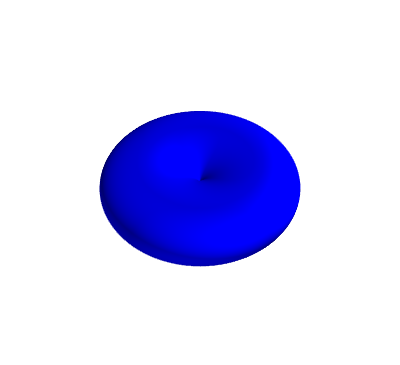
\includegraphics[scale=0.25]{sv0t},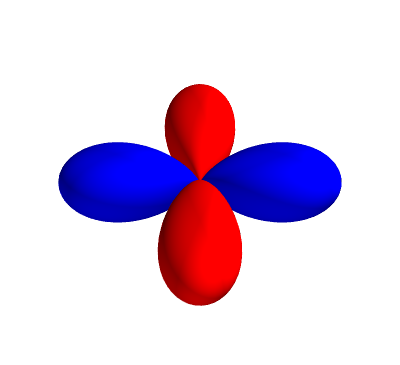
\includegraphics[scale=0.25]{sv1t}, 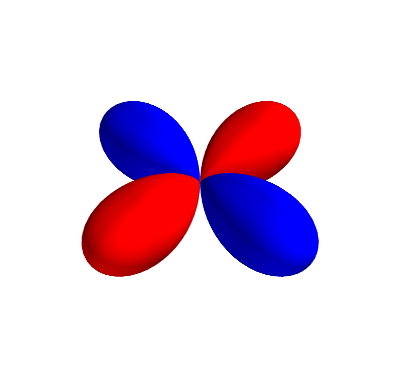
\includegraphics[scale=0.25]{sv2t}},
    xticklabel style={yshift=15pt},
    ] 
    \addplot+[
    ycomb,
    black,
    mark options={black}
    ] plot coordinates
	{(0,1.18) (1,0.59) (2,0.59)};
\end{axis}
\end{tikzpicture}
\end{document}
